\documentclass[11pt,a4paper]{article}

\usepackage[a4paper,margin=2.25cm]{geometry}
\usepackage{microtype}
\usepackage{parskip}
\usepackage{xcolor}
\usepackage{tabularx}
\usepackage{booktabs}
\usepackage{array}
\usepackage{colortbl}
\usepackage{enumitem}
\usepackage{titlesec}
\usepackage{fancyhdr}
\usepackage{lastpage}
\usepackage{hyperref}
\usepackage{xurl}
\usepackage{tikz}
\usepackage[most]{tcolorbox}
\usepackage{placeins}
\usepackage{float}
\usepackage{multicol}
\usetikzlibrary{arrows.meta,positioning,calc,shapes.geometric,matrix,fit,backgrounds}

\definecolor{deepblue}{RGB}{13,71,161}
\definecolor{medblue}{RGB}{25,118,210}
\definecolor{lightblue}{RGB}{227,242,253}
\definecolor{deepred}{RGB}{183,28,28}
\definecolor{lightred}{RGB}{255,235,238}
\definecolor{deepgreen}{RGB}{27,94,32}
\definecolor{lightgreen}{RGB}{232,245,233}
\definecolor{deeporange}{RGB}{230,81,0}
\definecolor{lightorange}{RGB}{255,243,224}
\definecolor{Ink}{HTML}{1F2937}
\definecolor{Muted}{HTML}{5B6472}
\definecolor{Line}{HTML}{B7C7DA}
\definecolor{Panel}{HTML}{F7FBFF}
\colorlet{Blue}{deepblue}
\colorlet{Green}{deepgreen}
\colorlet{Amber}{deeporange}
\colorlet{Rose}{deepred}

\hypersetup{
  colorlinks=true,
  linkcolor=Blue,
  urlcolor=Blue,
  citecolor=Blue,
  pdfauthor={BigChalkBox},
  pdftitle={BigChalkBox Pre-Seed Business Plan - Investor Edition}
}

\pagestyle{fancy}
\setlength{\headheight}{14.5pt}
\fancyhf{}
\fancyhead[L]{\small\textcolor{deepblue}{\textbf{BigChalkBox Pre-Seed Business Plan}}}
\fancyhead[R]{\small\textcolor{Muted}{Confidential \quad Page \thepage\ of \pageref{LastPage}}}
\fancyfoot[C]{\small\textcolor{Muted}{\textit{AI-native assessment infrastructure for Indian higher education}}}
\renewcommand{\headrulewidth}{0.6pt}
\renewcommand{\footrulewidth}{0pt}

\titleformat{\section}{\Large\bfseries\color{deepblue}}{\thesection.}{0.6em}{}[\titlerule]
\titleformat{\subsection}{\large\bfseries\color{medblue}}{\thesubsection.}{0.5em}{}
\titleformat{\subsubsection}{\normalsize\bfseries\color{deeporange}}{\thesubsubsection.}{0.4em}{}
\titlespacing{\section}{0pt}{1.15em}{0.55em}
\titlespacing{\subsection}{0pt}{0.95em}{0.35em}
\titlespacing{\subsubsection}{0pt}{0.75em}{0.25em}

\setlist[itemize]{leftmargin=1.25em,itemsep=0.2em,topsep=0.2em}
\setlist[enumerate]{leftmargin=1.4em,itemsep=0.2em,topsep=0.2em}
\renewcommand{\arraystretch}{1.22}

\newcolumntype{Y}{>{\raggedright\arraybackslash}X}
\newcolumntype{L}[1]{>{\raggedright\arraybackslash}p{#1}}
\newcommand{\rs}{INR}
\newcommand{\lac}{L}
\newcommand{\crore}{Cr}
\newcommand{\source}[2]{\href{#1}{#2}}

\newtcolorbox{callout}[1]{
  enhanced,
  breakable,
  colback=lightorange,
  colframe=deeporange,
  colbacktitle=deeporange,
  coltitle=white,
  fonttitle=\bfseries,
  title={#1},
  arc=4pt,
  boxrule=1.15pt,
  left=8pt,right=8pt,top=6pt,bottom=6pt,
  boxed title style={arc=3pt,boxrule=0pt},
  attach boxed title to top left={xshift=0pt,yshift=-0.1pt}
}

\newtcolorbox{bluebox}[1]{
  enhanced,breakable,colback=lightblue,colframe=deepblue,
  colbacktitle=deepblue,coltitle=white,fonttitle=\bfseries,
  title={#1},arc=4pt,boxrule=1.15pt,left=8pt,right=8pt,top=6pt,bottom=6pt,
  boxed title style={arc=3pt,boxrule=0pt},
  attach boxed title to top left={xshift=0pt,yshift=-0.1pt}
}

\newtcolorbox{greenbox}[1]{
  enhanced,breakable,colback=lightgreen,colframe=deepgreen,
  colbacktitle=deepgreen,coltitle=white,fonttitle=\bfseries,
  title={#1},arc=4pt,boxrule=1.15pt,left=8pt,right=8pt,top=6pt,bottom=6pt,
  boxed title style={arc=3pt,boxrule=0pt},
  attach boxed title to top left={xshift=0pt,yshift=-0.1pt}
}

\begin{document}

\begin{titlepage}
  \centering
  \vspace*{1.35cm}
  {\Huge\bfseries\color{deepblue} BigChalkBox\par}
  \vspace{0.28cm}
  {\Large\color{medblue} AI-Native Assessment Infrastructure for Indian Higher Education\par}
  \vspace{0.42cm}
  \rule{10.2cm}{0.7pt}
  \vspace{0.52cm}

  {\large\itshape Assessment generation \(\bullet\) moderation \(\bullet\) evaluation \(\bullet\) institutional intelligence\par}
  \vspace{0.95cm}

  
\begin{tikzpicture}
    \node[
      draw=deepblue,fill=lightblue,rounded corners=3mm,
      minimum width=12.8cm,minimum height=1.2cm,
      font=\bfseries\large,text=deepblue,line width=1.15pt,
      align=center
    ] {Pre-Seed Round: \rs\ 45,00,000 \quad | \quad 12-month execution plan};
  \end{tikzpicture}

  \vspace{1.05cm}
  {\Large\bfseries\color{Ink} Investor Business Plan\par}
  \vspace{0.25cm}
  {\large\color{Muted} Prepared for prospective investors\par}
  \vspace{0.35cm}
  {\large\color{Muted} August 2026\par}
  \vfill
  \begin{callout}{Confidentiality and forecast status}
    Prepared for prospective investors only. Not for distribution or reproduction without permission. Historical usage metrics are company-provided. Market sizing and financial projections are management estimates based on the assumptions stated in this document and are not guaranteed outcomes.
  \end{callout}
  \vspace{0.45cm}
  {\small \source{https://bigchalkbox.com}{bigchalkbox.com} \quad | \quad \source{https://www.dasesai.com}{dasesai.com}}
\end{titlepage}

\tableofcontents
\newpage

\section{Executive Summary}

BigChalkBox is building an AI-native operating layer for the academic assessment lifecycle. The platform generates and moderates assessments, evaluates handwritten and digital responses, and converts the resulting data into institutional intelligence and custom reports. Its core design advantage is a shared assessment record: the approved questions, sample answers, marking rubric, syllabus map, and evaluation results remain connected instead of being recreated at each step.

The company has been building and validating the platform with faculty since 2025. Company-reported testing includes 20+ educators, 100+ assessments generated or moderated, 24,000+ one-page digital assignments evaluated in one department deployment, and 1,000+ full multi-question answer scripts evaluated across smaller pilots. These figures represent product validation and pilot activity rather than recurring paid revenue.

\begin{bluebox}{Investment case in brief}
\begin{itemize}
  \item \textbf{Focused entry wedge:} assessment generation and moderation enter before the exam; DASES evaluation expands revenue after the exam.
  \item \textbf{Connected data advantage:} the same faculty-approved rubric powers creation, moderation, grading, feedback, and institutional reporting.
  \item \textbf{Visible monetisation:} usage-based assessment operations are complemented by recurring Academic Content Studio and Institutional Intelligence subscriptions.
  \item \textbf{Large but disciplined market:} a segmented \rs\ 1,561\crore\ TAM narrows to a \rs\ 362\crore\ serviceable market; the Year 3 base case captures approximately 1.1\% of SAM revenue.
  \item \textbf{Capital-efficient round:} \rs\ 45,00,000 funds product development, the core team, infrastructure, institutional deployments, and a repeatable proof case for the seed round.
\end{itemize}
\end{bluebox}

India's higher education system includes 1,289 registered universities and university-level institutions, 48,246 colleges, and 15,221 standalone institutions, with approximately 4.5 crore students in AISHE 2023-24.\footnote{Department of Higher Education, \textit{AISHE Final Report 2023-24}, released July 2026: \url{https://www.dohe-education.gov.in/static/uploads/2026/07/8616f33dfee644ab6b87a2bd0658b18d.pdf}.} BigChalkBox will commercialise through private universities and autonomous institutions that control assessment decisions, using a local reference deployment where founder access is strongest before expanding to NCR and other private higher-education clusters.

\begin{callout}{The round}
BigChalkBox is raising \textbf{\rs\ 45,00,000} to complete production-grade assessment workflows, add engineering and delivery capacity, strengthen cloud/security infrastructure, and convert pilots into paid institutional deployments. The operating objective is a 12-month runway ending with a validated university deployment, measured unit economics, and a seed-ready operating data room.
\end{callout}

\section{The Problem}

Indian universities run repeated assessment cycles across mid-terms, end-terms, internal exams, assignments, practicals, and re-evaluation windows. Four workflows remain fragmented:

\begin{itemize}
  \item \textbf{Assessment design is inconsistent.} Faculty manually draft papers, while syllabus coverage, course-outcome mapping, difficulty balance, and Bloom's-level distribution are rarely checked systematically before release.
  \item \textbf{Moderation is slow and subjective.} A second faculty member often reviews the assessment manually, adding time without creating a reusable record of the quality checks performed.
  \item \textbf{Evaluation does not scale.} Descriptive answer evaluation is slow and inconsistent across evaluators, delaying results and limiting actionable feedback for students.
  \item \textbf{Leadership sees marks, not learning signals.} Academic leaders typically receive final scores without a structured view of weak concepts, prerequisite gaps, assessment-quality trends, or teaching-assessment misalignment.
\end{itemize}

NEP 2020 and outcome-based education frameworks increase the need for auditable academic processes. UGC's Curriculum and Credit Framework for Undergraduate Programmes links curriculum design, learning outcomes, flexible credits, and student-centric delivery.\footnote{UGC Curriculum and Credit Framework: \url{https://www.ugc.gov.in/KeyInitiative}; Department of Higher Education, NEP 2020: \url{https://www.dohe-education.gov.in/department/nep/details/national-education-policy-2020-QzN1IzMtQWa}.} Assessment quality is therefore an institutional management issue, not only a faculty workload issue.

\section{The BigChalkBox Product Architecture}

BigChalkBox separates the product into three commercial layers with one shared data model.

\subsection{Assessment Operations}

\subsubsection{Assessment Generation: \rs\ 400 + GST per assessment}
\begin{itemize}
  \item End-to-end AI generation aligned to syllabus, section structure, difficulty, course outcomes, and Bloom's levels.
  \item Sample answers for every question and marking rubrics with criterion descriptors.
  \item Print-ready output in the institution's required format.
\end{itemize}

\subsubsection{Assessment Moderation: \rs\ 400 + GST per assessment}
\begin{itemize}
  \item AI-assisted review for syllabus coverage, ambiguity, gaps, overlaps, difficulty balance, and Bloom's verification.
  \item Structured moderation record for academic-quality and accreditation workflows.
  \item Sample answers and marking rubrics scheduled for the September 2026 release.
\end{itemize}

\subsubsection{DASES Evaluation}
\begin{itemize}
  \item \textbf{Handwritten answer booklet evaluation: \rs\ 40 + GST per full booklet.} The standard operating model includes the special printed booklet, scanning workflow, rubric-linked scoring, question-level feedback, and faculty review.
  \item \textbf{Digital Text Evaluation: \rs\ 25 + GST per student per course.} The institution uploads typed responses; DASES produces per-question scores and feedback against the approved rubric.
  \item Question-level results preserve the link to the approved assessment, sample answers, and marking criteria.
\end{itemize}

\subsection{Academic Content Studio}

The Academic Content Studio converts approved curricula into institution-controlled teaching assets: lecture-level plans, faculty notes, in-class quizzes, practice sets, prerequisite refreshers, and student Q\&A constrained to approved course material.

\begin{itemize}
  \item \textbf{Department plan: \rs\ 60,000 + GST per year} for up to 10 active courses and 5,000 pooled student Q\&A queries.
  \item \textbf{Institution plan: \rs\ 1,50,000 + GST per year} for up to 50 active courses and 25,000 pooled student Q\&A queries.
  \item \textbf{Enterprise plan: custom quote + GST} for larger course and query pools, integrations, and dedicated support.
\end{itemize}

\subsection{Institutional Intelligence and Custom Reports}

This separate subscription turns curriculum, assessment, evaluation, and Q\&A activity into decision support for deans, Controllers of Examination, IQAC teams, and academic leadership. Outputs include weak-topic analysis, prerequisite gaps, difficulty and outcome-mapping trends, cross-section comparison, assessment-teaching mismatch, and institution-specific custom reports.

\begin{itemize}
  \item \textbf{Institution plan: \rs\ 2,00,000 + GST per year} for up to 10 departments, standard dashboards, and quarterly custom reports.
  \item \textbf{Enterprise plan: custom quote + GST} for additional departments, ERP/LMS integration, advanced data pipelines, and bespoke reporting cycles.
\end{itemize}

\begin{greenbox}{Why pooled institutional pricing solves course-size volatility}
The subscription is not charged separately for every course or every enrolled student. Each institution buys an annual pool of active-course capacity and student Q\&A usage. A four-student course consumes little of the pool; a 2,000-student course consumes more but benefits from declining-volume query packs. Large contracts retain a minimum contribution-margin floor, while Digital Text Evaluation remains a transparent \rs\ 25 + GST per student-course usage charge. This preserves adoption for small courses without making large cohorts prohibitively expensive.
\end{greenbox}

\begin{figure}[H]
\centering
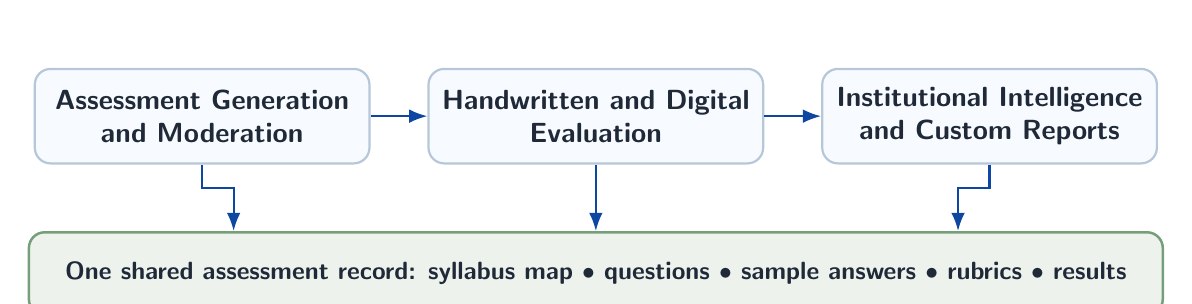
\begin{tikzpicture}[
  stage/.style={draw=Line,fill=Panel,rounded corners=2mm,minimum width=4.25cm,minimum height=1.20cm,align=center,font=\sffamily\bfseries,text=Ink,line width=0.8pt},
  spine/.style={draw=Green!60,fill=Green!8,rounded corners=2mm,minimum width=14.4cm,minimum height=1.05cm,align=center,font=\sffamily\small\bfseries,text=Ink,line width=0.9pt},
  arrow/.style={-Latex,thick,color=Blue}
]
\node[stage] (design) at (-5.0,0) {Assessment Generation\\and Moderation};
\node[stage] (evaluate) at (0,0) {Handwritten and Digital\\Evaluation};
\node[stage] (insight) at (5.0,0) {Institutional Intelligence\\and Custom Reports};
\node[spine] (record) at (0,-2.0) {One shared assessment record: syllabus map \(\bullet\) questions \(\bullet\) sample answers \(\bullet\) rubrics \(\bullet\) results};

\draw[arrow] (design.east) -- (evaluate.west);
\draw[arrow] (evaluate.east) -- (insight.west);
\draw[arrow] (design.south) -- ++(0,-0.30) -| ([xshift=-4.6cm]record.north);
\draw[arrow] (evaluate.south) -- (record.north);
\draw[arrow] (insight.south) -- ++(0,-0.30) -| ([xshift=4.6cm]record.north);
\end{tikzpicture}
\caption{BigChalkBox connects pre-exam quality, post-exam evaluation, and institutional decision support through one governed assessment record.}
\end{figure}
\FloatBarrier

\section{Traction and Validation}

\begin{tabularx}{\textwidth}{>{\bfseries}p{0.20\textwidth}Y}
\toprule
20+ educators & Faculty members have tested assessment or evaluation workflows. \\
100+ assessments & Assessments generated or moderated during company testing. \\
24,000+ digital assignments & One-page typed assignments evaluated in a high-volume department deployment. \\
1,000+ full answer scripts & Multi-question evaluation runs closer to the core university exam use case. \\
500-sheet parallel capacity & Current DASES product claim; approximately 15 seconds per sheet in the published workflow. \\
\bottomrule
\end{tabularx}

The traction mix matters. The 24,000+ one-page assignments validate throughput, while the 1,000+ full scripts test the more demanding multi-question use case. The immediate commercial objective is to convert this technical validation into repeatable, paid institutional usage.\footnote{Company-provided pilot metrics as at August 2026. Published product claims are available at \url{https://www.dasesai.com/} and \url{https://www.dasesai.com/about}.}

\section{Market Opportunity}

\subsection{TAM: a segmented Indian higher-education budget pool}

The TAM uses four non-overlapping client segments and segment-specific annual spend assumptions. GST is excluded because it is collected on behalf of the government and is not revenue. Autonomous colleges are separated from the wider college universe to avoid double counting.

\begin{tabularx}{\textwidth}{L{0.21\textwidth}>{\raggedleft\arraybackslash}p{0.12\textwidth}L{0.38\textwidth}>{\raggedleft\arraybackslash}p{0.14\textwidth}}
\toprule
\textbf{Client segment} & \textbf{Count} & \textbf{Annual spend assumption} & \textbf{TAM} \\
\midrule
Universities and university-level institutions & 1,289 & \rs\ 20L evaluation capacity + \rs\ 4L assessment, content, and intelligence = \rs\ 24L & \rs\ 309\crore \\
Autonomous colleges & 1,300 & \rs\ 8L evaluation capacity + \rs\ 2L software layers = \rs\ 10L & \rs\ 130\crore \\
Other colleges & 46,946 & 5,000 digital student-course evaluations + assessment/content tools = \rs\ 2L & \rs\ 939\crore \\
Standalone institutions & 15,221 & 2,500 digital student-course evaluations + core tools = \rs\ 1.2L & \rs\ 183\crore \\
\midrule
\textbf{Total TAM} & \textbf{64,756} & \textbf{Sum of segment budget pools} & \textbf{\rs\ 1,561\crore} \\
\bottomrule
\end{tabularx}

Institution counts come from AISHE 2023-24, except the 1,300 autonomous-college planning count, which is based on the current UGC public list and rounded for modelling.\footnote{UGC autonomous college list: \url{https://www.ugc.gov.in/colleges/Autonomous_Colleges_list}. The count is a planning approximation and should be refreshed before a formal financing close.}

\subsection{SAM: institutions with purchasing control and early-adopter fit}

The serviceable market narrows the same TAM segments rather than applying a new ARPU. It includes 546 private unaided universities, approximately 1,300 autonomous colleges, 10\% of private unaided responding colleges as an early-adopter filter, and 3,000 priority standalone professional institutions. AISHE reports that 70\% of responding colleges are private unaided. The 10\% and 3,000 filters are management assumptions, clearly separated from published facts.

\begin{tabularx}{\textwidth}{L{0.36\textwidth}>{\raggedleft\arraybackslash}p{0.15\textwidth}>{\raggedleft\arraybackslash}p{0.20\textwidth}Y}
\toprule
\textbf{SAM segment} & \textbf{Institutions} & \textbf{Annual spend} & \textbf{SAM value} \\
\midrule
Private unaided universities & 546 & \rs\ 24L & \rs\ 131\crore \\
Autonomous colleges & 1,300 & \rs\ 10L & \rs\ 130\crore \\
Early-adopter private colleges & 3,253 & \rs\ 2L & \rs\ 65\crore \\
Priority standalone institutions & 3,000 & \rs\ 1.2L & \rs\ 36\crore \\
\midrule
\textbf{Total SAM} & \textbf{8,099} & & \textbf{\rs\ 362\crore} \\
\bottomrule
\end{tabularx}

\subsection{SOM: Year 3 base case}

The Year 3 operating target is 10 active university customers plus selective subscription adoption and small non-university validation revenue. The corresponding base-case revenue is \rs\ 3.98\crore, equal to approximately 1.1\% of the \rs\ 362\crore\ SAM. This is a revenue-based SOM; customer penetration is approximately 0.12\% of the 8,099 SAM institutions.

\begin{figure}[H]
\centering
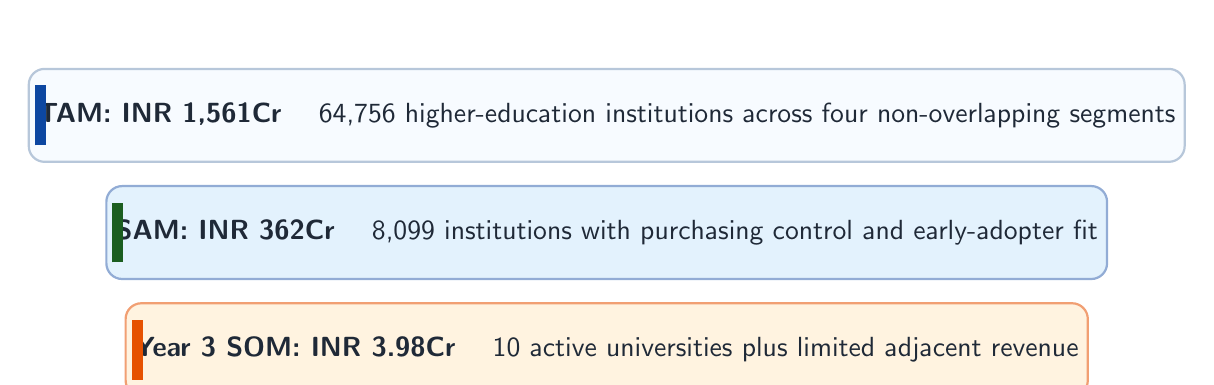
\begin{tikzpicture}[
  market/.style={draw=Line,fill=Panel,rounded corners=2mm,minimum height=1.18cm,align=left,text=Ink,font=\sffamily,line width=0.8pt},
  tam/.style={market,minimum width=14.2cm},
  sam/.style={market,minimum width=10.2cm,fill=lightblue,draw=Blue!45},
  som/.style={market,minimum width=7.2cm,fill=lightorange,draw=Amber!55}
]
\node[tam] (t) {\textbf{TAM: \rs\ 1,561\crore} \quad 64,756 higher-education institutions across four non-overlapping segments};
\node[sam,below=0.28cm of t] (s) {\textbf{SAM: \rs\ 362\crore} \quad 8,099 institutions with purchasing control and early-adopter fit};
\node[som,below=0.28cm of s] (o) {\textbf{Year 3 SOM: \rs\ 3.98\crore} \quad 10 active universities plus limited adjacent revenue};
\draw[Blue,line width=4pt,rounded corners=2pt] ([xshift=0.16cm,yshift=-0.38cm]t.west) -- ([xshift=0.16cm,yshift=0.38cm]t.west);
\draw[Green,line width=4pt,rounded corners=2pt] ([xshift=0.16cm,yshift=-0.38cm]s.west) -- ([xshift=0.16cm,yshift=0.38cm]s.west);
\draw[Amber,line width=4pt,rounded corners=2pt] ([xshift=0.16cm,yshift=-0.38cm]o.west) -- ([xshift=0.16cm,yshift=0.38cm]o.west);
\end{tikzpicture}
\caption{A consistent segment model keeps SAM below TAM and ties SOM directly to the operating forecast.}
\end{figure}
\FloatBarrier

\section{Business Model and Pricing}

BigChalkBox uses a three-part revenue model: transactional Assessment Operations, a pooled Academic Content Studio licence, and a separate Institutional Intelligence subscription. All list prices below are exclusive of GST.

\begin{tabularx}{\textwidth}{L{0.29\textwidth}L{0.24\textwidth}Y}
\toprule
\textbf{Product} & \textbf{List price} & \textbf{Commercial role} \\
\midrule
Assessment Generation & \rs\ 400 + GST / assessment & Low-friction entry into the pre-exam workflow. \\
Assessment Moderation & \rs\ 400 + GST / assessment & Quality and audit layer before release. \\
Handwritten evaluation & \rs\ 40 + GST / full booklet & High-volume evaluation and feedback workflow. \\
Digital Text Evaluation & \rs\ 25 + GST / student / course & Software-led evaluation for typed responses. \\
Academic Content Studio & \rs\ 60,000 or \rs\ 1.50L + GST / year & Recurring department or institution licence with pooled course and query capacity. \\
Institutional Intelligence and Custom Reports & \rs\ 2.00L + GST / year & Separate analytics and reporting subscription for academic leadership. \\
Enterprise deployment & Custom quote + GST & Larger pools, integrations, SLAs, and bespoke reporting. \\
\bottomrule
\end{tabularx}

Assessment Generation and Moderation are intentionally accessible entry products. Evaluation creates volume revenue, while the two software subscriptions increase recurring revenue and blended gross margin after institutional trust is established.

\section{Competitive Landscape}

The market includes broad exam platforms, specialist evaluation infrastructure, and grading tools. BigChalkBox's position is not that competitors are absent; it is that pre-exam quality, post-exam evaluation, and institution-level insight are connected through one assessment record and sold with India-specific deployment support.

\begin{tabularx}{\textwidth}{L{0.16\textwidth}L{0.25\textwidth}L{0.26\textwidth}Y}
\toprule
\textbf{Player} & \textbf{Public positioning} & \textbf{Overlap with BigChalkBox} & \textbf{BigChalkBox differentiation} \\
\midrule
CodeTantra & Broad academic ERP, LMS, online/proctored exams, question-paper management, and on-screen digital evaluation & Strong institutional exam workflow and established distribution & AI-native shared rubric from assessment design through evaluation; focused deployment and transparent usage pricing. \\
CrazyGoldFish & Multimodal evaluation infrastructure, learning signals, APIs, personalisation, and a persistent learning-memory layer & Direct overlap in rubric-based handwritten/digital evaluation and downstream insight & Owns the pre-exam generation and moderation workflow; operational fit for Indian university paper-based exams. \\
Eklavvya & Online exams, remote proctoring, and on-screen evaluation & Exam delivery, evaluation workflow, and institutional procurement & Descriptive-answer AI evaluation linked to faculty-approved sample answers, rubrics, and assessment-quality records. \\
Gradescope & Rubric-assisted grading and course-level assessment workflows in global higher education & Faculty grading productivity and rubric workflows & INR pricing, Indian descriptive-exam formats, handwriting pipeline, local deployment, and institutional custom reports. \\
\bottomrule
\end{tabularx}

CodeTantra publicly describes support for online and blended assessments, handwritten uploads, programming questions, question-paper management, answer-booklet printing, and digital evaluation. CrazyGoldFish positions itself as evaluation infrastructure spanning handwriting, typed responses, diagrams, audio, and video, with structured learning signals and human review.\footnote{CodeTantra product evidence: \url{https://play.google.com/store/apps/details?id=com.codetantra.seam} and the Didac India 2025 catalogue at \url{https://didacindia.com/}. CrazyGoldFish: \url{https://crazygoldfish.com/} and \url{https://docs.crazygoldfish.com/products/evaluation-layer-overview}. Eklavvya: \url{https://www.eklavvya.com/}. Gradescope: \url{https://www.gradescope.com/}.}

\section{Go-To-Market Strategy}

\subsection{Land with a paid assessment deployment}

The first paid reference will be pursued where the founders have the strongest access to academic leadership, including Dehradun and the wider Uttarakhand higher-education cluster. The initial deployment targets 2-3 programs, a defined assessment window, faculty-approved rubrics, and pre-agreed success metrics for turnaround, scoring agreement, exception rate, and unit cost.

\subsection{Expand within the institution}

After the first successful evaluation cycle, BigChalkBox expands along two paths: more programs and assessment volumes inside DASES; and recurring adoption of Academic Content Studio plus Institutional Intelligence and Custom Reports. The shared assessment record reduces implementation friction because the institution does not need to rebuild course, rubric, or outcome data for each module.

\subsection{Replicate through reference-led institutional sales}

Year 2 prioritises private universities and autonomous institutions in NCR and nearby markets where a credible reference can shorten diligence. Year 3 adds selected private-education clusters in Maharashtra, Karnataka, Telangana, Tamil Nadu, and the Gujarat-Rajasthan belt. Premium-school and coaching pilots remain controlled discovery channels rather than a primary forecast engine.

\begin{bluebox}{Sales motion and proof required}
Paid pilot \(\rightarrow\) faculty acceptance and cost benchmark \(\rightarrow\) program expansion \(\rightarrow\) university-wide evaluation \(\rightarrow\) content and intelligence subscriptions. Each stage has a clear buyer, deployment scope, success metric, and expansion decision.
\end{bluebox}

\section{Financial Projections}

The base case models one active university in Year 1, four in Year 2, and ten in Year 3. Revenue excludes GST. Handwritten evaluation volumes represent paid assessment cycles, not total institutional examination volume. Premium-school and coaching revenue is deliberately limited to \rs\ 0.25L, \rs\ 0.50L, and \rs\ 1.00L across the three years.

\subsection{Operating drivers}

\begin{tabularx}{\textwidth}{Y>{\raggedleft\arraybackslash}p{0.17\textwidth}>{\raggedleft\arraybackslash}p{0.17\textwidth}>{\raggedleft\arraybackslash}p{0.17\textwidth}}
\toprule
\textbf{Driver} & \textbf{Year 1} & \textbf{Year 2} & \textbf{Year 3} \\
\midrule
Active universities & 1 & 4 & 10 \\
Handwritten booklets & 45,000 & 285,000 & 870,000 \\
Digital student-course evaluations & 0 & 20,000 & 80,000 \\
Assessment Generation / Moderation transactions & 250 & 1,000 & 3,000 \\
Academic Content Studio subscriptions & 1 department & 4 departments & 6 institutions \\
Institutional Intelligence subscriptions & 0 & 1 institution & 4 institutions \\
\bottomrule
\end{tabularx}

\begin{greenbox}{How the handwritten volumes are derived}
\textbf{Year 1:} 1 new paid pilot \(\times\) 45,000 booklets = 45,000.\par
\textbf{Year 2:} 1 expansion cycle \(\times\) 150,000 + 3 new pilots \(\times\) 45,000 = 285,000.\par
\textbf{Year 3:} 4 expansion cycles \(\times\) 150,000 + 6 new pilots \(\times\) 45,000 = 870,000.
\end{greenbox}

\subsection{Revenue and gross profit bridge}

\begin{tabularx}{\textwidth}{Y>{\raggedleft\arraybackslash}p{0.17\textwidth}>{\raggedleft\arraybackslash}p{0.17\textwidth}>{\raggedleft\arraybackslash}p{0.17\textwidth}}
\toprule
\textbf{Revenue line} & \textbf{Year 1} & \textbf{Year 2} & \textbf{Year 3} \\
\midrule
Handwritten evaluation at \rs\ 40 / booklet & \rs\ 18.00L & \rs\ 114.00L & \rs\ 348.00L \\
Digital Text Evaluation at \rs\ 25 / student-course & \rs\ 0.00L & \rs\ 5.00L & \rs\ 20.00L \\
Assessment Generation / Moderation at \rs\ 400 / transaction & \rs\ 1.00L & \rs\ 4.00L & \rs\ 12.00L \\
Academic Content Studio subscriptions & \rs\ 0.60L & \rs\ 2.40L & \rs\ 9.00L \\
Institutional Intelligence subscriptions & \rs\ 0.00L & \rs\ 2.00L & \rs\ 8.00L \\
School / coaching validation revenue & \rs\ 0.25L & \rs\ 0.50L & \rs\ 1.00L \\
\midrule
\textbf{Total revenue} & \textbf{\rs\ 19.85L} & \textbf{\rs\ 127.90L} & \textbf{\rs\ 398.00L} \\
Direct delivery costs & \rs\ 10.15L & \rs\ 65.85L & \rs\ 203.95L \\
\textbf{Gross profit} & \textbf{\rs\ 9.70L} & \textbf{\rs\ 62.05L} & \textbf{\rs\ 194.05L} \\
\textbf{Gross margin} & \textbf{48.9\%} & \textbf{48.5\%} & \textbf{48.8\%} \\
\bottomrule
\end{tabularx}

The total is the sum of the six revenue lines. For example, Year 3 equals \rs\ 348.00L + \rs\ 20.00L + \rs\ 12.00L + \rs\ 9.00L + \rs\ 8.00L + \rs\ 1.00L = \rs\ 398.00L. Gross profit subtracts product-level direct costs described in the next section; it is not EBITDA and excludes central payroll, sales, legal, rent, corporate cloud overhead, and financing costs.

\begin{figure}[H]
\centering
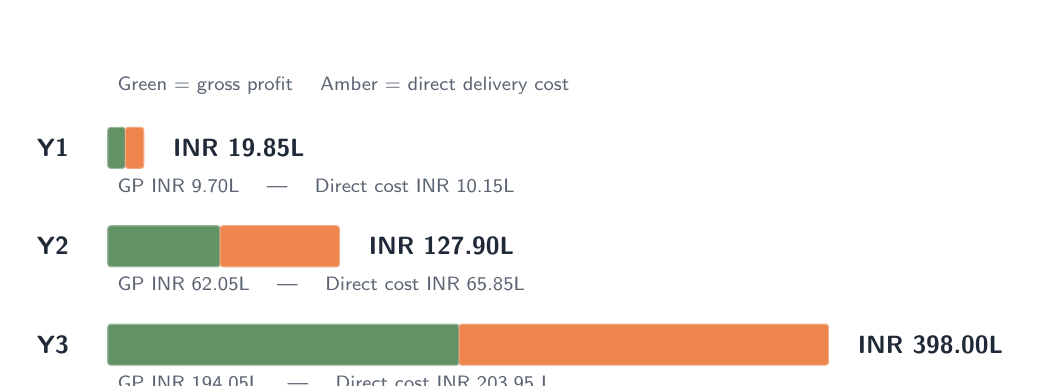
\begin{tikzpicture}[
  bar/.style={rounded corners=1pt},
  year/.style={font=\sffamily\bfseries\small,text=Ink,anchor=east},
  val/.style={font=\sffamily\bfseries\small,text=Ink,anchor=west},
  note/.style={font=\sffamily\scriptsize,text=Muted,anchor=west}
]
\node[note] at (1.45,1.05) {Green = gross profit \quad Amber = direct delivery cost};
\foreach \y/\label/\rev/\gp/\cost in {
  0/Y1/19.85/9.70/10.15,
  -1.25/Y2/127.90/62.05/65.85,
  -2.50/Y3/398.00/194.05/203.95
} {
  \pgfmathsetmacro{\gpw}{\gp*0.023}
  \pgfmathsetmacro{\costw}{\cost*0.023}
  \node[year] at (1.08,\y+0.26) {\label};
  \draw[bar,fill=Green!68,draw=Green!45] (1.45,\y) rectangle ++(\gpw,0.52);
  \draw[bar,fill=Amber!70,draw=Amber!50] (1.45+\gpw,\y) rectangle ++(\costw,0.52);
  \node[val] at (1.70+\gpw+\costw,\y+0.26) {\rs\ \rev L};
  \node[note] at (1.45,\y-0.22) {GP \rs\ \gp L \quad | \quad Direct cost \rs\ \cost L};
}
\end{tikzpicture}
\caption{Revenue and direct-cost bridge. The lower initial margin reflects printing, scanning, and model costs in handwritten evaluation; the software subscriptions improve mix over time.}
\end{figure}
\FloatBarrier

\section{Unit Economics and Direct Costs}

All contribution figures exclude GST. The model uses standard Gemini 3.5 Flash-Lite pricing of US\$0.30 per million input tokens and US\$2.50 per million output tokens, converted at \rs\ 96.25 per US dollar.\footnote{Google Gemini Developer API pricing, last updated July 2026: \url{https://ai.google.dev/gemini-api/docs/pricing}. Direct-cost estimates also include non-model delivery items and are management assumptions to be validated during paid deployments.}

\begin{tabularx}{\textwidth}{L{0.28\textwidth}>{\raggedleft\arraybackslash}p{0.16\textwidth}>{\raggedleft\arraybackslash}p{0.16\textwidth}>{\raggedleft\arraybackslash}p{0.16\textwidth}Y}
\toprule
\textbf{Product unit} & \textbf{Revenue} & \textbf{Direct cost} & \textbf{Gross profit} & \textbf{GM} \\
\midrule
Assessment Generation & \rs\ 400 & \rs\ 30 & \rs\ 370 & 92.5\% \\
Assessment Moderation & \rs\ 400 & \rs\ 25 & \rs\ 375 & 93.8\% \\
Handwritten full booklet & \rs\ 40 & \rs\ 22 & \rs\ 18 & 45.0\% \\
Digital text, student-course & \rs\ 25 & \rs\ 10 & \rs\ 15 & 60.0\% \\
Content Studio institution-year & \rs\ 1.50L & \rs\ 0.32L & \rs\ 1.18L & 78.7\% \\
Intelligence institution-year & \rs\ 2.00L & \rs\ 0.35L & \rs\ 1.65L & 82.5\% \\
\bottomrule
\end{tabularx}

\subsection{Cost build by product}

\begin{tabularx}{\textwidth}{L{0.30\textwidth}Y}
\toprule
\textbf{Product} & \textbf{Direct-cost build} \\
\midrule
Assessment Generation & Two-pass standard-model workflow using approximately 120,000 input and 40,000 output tokens per pass, plus formatting and storage; modelled total \rs\ 30. \\
Assessment Moderation & Two-pass review using approximately 100,000 input and 25,000 output tokens per pass, plus report formatting and storage; modelled total \rs\ 25. \\
Handwritten evaluation & \rs\ 12 model/API + \rs\ 6 printed booklet + \rs\ 4 scanning labour, QA, storage, and exception handling = \rs\ 22. \\
Digital Text Evaluation & Company-provided direct cost of \rs\ 10 per student-course, including model processing and delivery infrastructure. \\
Academic Content Studio & Up to 50 course setups at approximately \rs\ 150 each after a two-pass generation/QA workflow; 2,500 active learners averaging 10 queries each creates the 25,000-query pool, with 2,000 input and 500 output tokens per query; retrieval, monitoring, usage variance, and direct support produce a modelled annual cost of \rs\ 32,000. \\
Institutional Intelligence & Data processing, scheduled analysis, quarterly custom report generation, storage, and direct report QA produce a modelled annual direct cost of \rs\ 35,000 for the standard institution plan. \\
\bottomrule
\end{tabularx}

The raw model cost for a typical university course setup is approximately \rs\ 57 for one pass at the cited Gemini rate, or about \rs\ 114 for two passes; the model rounds this to \rs\ 150 after formatting and storage. A 25,000-query pool at the stated query-token assumption has raw model cost of approximately \rs\ 4,450. The larger \rs\ 32,000 subscription direct-cost provision covers retrieval, monitoring, usage variance, course setup, and direct support rather than treating token cost as the entire cost of delivery.

\begin{callout}{Margin expansion levers}
The current base case is intentionally conservative because handwritten evaluation includes physical operations. Margin can improve through institution-operated scanning, negotiated booklet printing, rubric-context caching, batch inference, lower exception rates, and a higher mix of Digital Text Evaluation, Academic Content Studio, and Institutional Intelligence subscriptions. The model does not assume these savings in the three-year gross-profit forecast.
\end{callout}

\section{Team and Operating Plan}

BigChalkBox has been operating since 2025 with a founder-led team combining product development, education relationships, and AI evaluation engineering.

\begin{tabularx}{\textwidth}{L{0.27\textwidth}L{0.25\textwidth}Y}
\toprule
\textbf{Name} & \textbf{Role} & \textbf{Relevant responsibility} \\
\midrule
\textbf{Konal Puri} & Co-founder / CEO & Product direction, institutional relationships, commercial development, and faculty validation. \\
Co-founder name available in investor data room & Co-founder / CTO & AI evaluation pipeline, platform engineering, workflow reliability, and data infrastructure. \\
\bottomrule
\end{tabularx}

The round adds focused capacity around the founders: two product/AI engineers, one institutional sales lead, and shared academic QA/customer-success and deployment-operations support. Hiring is milestone-led; the company does not plan a broad functional build before paid institutional proof.

\section{The Round and Use of Funds}

BigChalkBox is raising \textbf{\rs\ 45,00,000}, approximately \textbf{US\$46,753} at \textbf{\rs\ 96.25 per US dollar}.\footnote{RBI exchange-rate display: \rs\ 96.2537 per US dollar at 1:00 p.m. on 21 July 2026, available through \url{https://www.rbi.org.in/}. The document uses \rs\ 96.25 for presentation.} The financing is intended as a 12-month pre-seed execution round. Final security, valuation, and conversion terms will be agreed with the lead investor and transaction counsel.

\subsection{Use of funds}

\begingroup
\small
\renewcommand{\arraystretch}{1.08}
\begin{tabularx}{\textwidth}{L{0.28\textwidth}>{\raggedleft\arraybackslash}p{0.14\textwidth}>{\raggedleft\arraybackslash}p{0.11\textwidth}Y}
\toprule
\textbf{Category} & \textbf{Amount} & \textbf{Share} & \textbf{Execution outcome} \\
\midrule
Product and AI engineering & \rs\ 16.0L & 35.6\% & Production-grade generation, moderation, evaluation reliability, QA tooling, integrations, and September 2026 rubric/sample-answer releases. \\
Core team and delivery capacity & \rs\ 10.0L & 22.2\% & Two engineering contributors plus academic QA, customer-success, and deployment support around the founders. \\
Institutional GTM and pilot acquisition & \rs\ 7.0L & 15.6\% & Target-account outreach, paid-pilot conversion, travel, demos, proposals, and reference-led sales. \\
Cloud, model API, security, and data infrastructure & \rs\ 5.5L & 12.2\% & Hosting, inference, observability, backups, access controls, security review, and India-oriented data architecture. \\
Deployment hardware and working capital & \rs\ 3.5L & 7.8\% & Scanners, pilot printing, site setup, payment-timing buffer, and controlled delivery capacity. \\
Legal, finance, administration, and contingency & \rs\ 3.0L & 6.7\% & Company compliance, accounting, contracts, insurance, and execution contingency. \\
\midrule
\textbf{Total} & \textbf{\rs\ 45.0L} & \textbf{100.0\%} & \textbf{12-month pre-seed plan.} \\
\bottomrule
\end{tabularx}
\endgroup

\subsection{Milestones financed by the round}

\begin{enumerate}
  \item Ship production-ready Assessment Generation, Assessment Moderation, DASES evaluation, and the first subscription-ready Academic Content Studio workflows.
  \item Convert at least one university to a paid assessment deployment and process a first paid cycle of up to 45,000 handwritten booklets.
  \item Complete a faculty-audited reliability benchmark covering scoring agreement, exception rate, feedback quality, processing time, and dispute handling.
  \item Validate the full \rs\ 22 direct-cost build per handwritten booklet and the \rs\ 10 cost per Digital Text Evaluation student-course.
  \item Establish a repeatable second-institution pipeline and package the first deployment into an investor-grade case study and seed data room.
\end{enumerate}

\section{Key Risks and Mitigants}

\begin{tabularx}{\textwidth}{L{0.30\textwidth}Y}
\toprule
\textbf{Risk} & \textbf{Mitigant} \\
\midrule
Long university sales and procurement cycles & Use a tightly scoped paid pilot with defined academic and financial success metrics, then expand through reference-led selling. \\
Trust in AI-assisted grading & Preserve faculty authority, rubric provenance, question-level evidence, human review, exceptions, and a complete dispute audit trail. \\
45\% handwritten gross margin is below software benchmarks & Make physical costs visible; support institution-operated scanning; improve print procurement, batching, caching, and software subscription mix. \\
On-site scanning complexity & Standardise answer booklets, benchmark throughput, maintain batch controls, and stage rollout by assessment window and program. \\
Established exam and evaluation competitors & Compete on the connected pre-exam-to-insight workflow, India-specific deployment, and transparent usage economics rather than claiming feature exclusivity. \\
Data privacy and security requirements & Use access controls, encryption, logging, retention/deletion policies, India-oriented hosting posture, and a funded security workstream. \\
Small-team execution risk & Tie hiring to funded milestones and add focused engineering, sales, academic QA, and deployment capacity around the founders. \\
Subscription adoption remains unproven & Keep subscription revenue assumptions modest, separate content from intelligence pricing, and sell both only after assessment workflows establish institutional trust. \\
\bottomrule
\end{tabularx}

\section{Appendix: Assumptions and Source Notes}

\subsection{Facts, company data, and management assumptions}

\begin{itemize}
  \item \textbf{Company-provided:} founding timeline, pilot volumes, 100+ assessment generation/moderation count, prices, product roadmap, direct API cost of \rs\ 12 per handwritten booklet, and direct cost of \rs\ 10 per Digital Text Evaluation student-course.
  \item \textbf{Public sources:} AISHE institution and enrolment counts; UGC autonomous college list; competitor public product descriptions; Gemini API prices; RBI exchange-rate display.
  \item \textbf{Management assumptions:} segment annual spend, early-adopter filters, forecast conversion and volume, subscription adoption, token workloads, non-API direct costs, school/coaching validation revenue, and all projected financial outcomes.
\end{itemize}

\subsection{Source register}

\begingroup
\small
\begin{multicols}{2}
\begin{itemize}
  \setlength{\itemsep}{0.08em}
  \item AISHE 2023-24: \source{https://www.dohe-education.gov.in/static/uploads/2026/07/8616f33dfee644ab6b87a2bd0658b18d.pdf}{Department of Higher Education final report}.
  \item UGC autonomous colleges: \source{https://www.ugc.gov.in/colleges/Autonomous_Colleges_list}{UGC public list}.
  \item NEP and UGC context: \source{https://www.dohe-education.gov.in/department/nep/details/national-education-policy-2020-QzN1IzMtQWa}{NEP 2020} and \source{https://www.ugc.gov.in/KeyInitiative}{UGC key initiatives}.
  \item DASES product: \source{https://www.dasesai.com/}{product site}, \source{https://www.dasesai.com/about}{company/product metrics}, and \source{https://www.dasesai.com/solutions}{solution architecture}.
  \item CodeTantra: \source{https://play.google.com/store/apps/details?id=com.codetantra.seam}{official Android app description} and \source{https://didacindia.com/}{Didac India exhibitor catalogue}.
  \item CrazyGoldFish: \source{https://crazygoldfish.com/}{company site} and \source{https://docs.crazygoldfish.com/products/evaluation-layer-overview}{evaluation-layer documentation}.
  \item Eklavvya and Gradescope: \source{https://www.eklavvya.com/}{Eklavvya} and \source{https://www.gradescope.com/}{Gradescope}.
  \item Gemini pricing: \source{https://ai.google.dev/gemini-api/docs/pricing}{Google AI for Developers}.
  \item USD/INR reference: \source{https://www.rbi.org.in/}{Reserve Bank of India}.
\end{itemize}
\end{multicols}
\endgroup

\begin{callout}{Investor diligence items}
Before a financing close, BigChalkBox will provide the detailed pilot ledger, faculty validation evidence, product-security documentation, customer pipeline, legal entity and cap-table documents, and a monthly cash plan. Forecasts in this business plan should be read alongside those diligence materials.
\end{callout}

\end{document}
